\documentclass[11pt,a4paper]{article}
\usepackage[utf8]{inputenc}
\usepackage[T1]{fontenc}
\usepackage{amsmath,amssymb,amsfonts}
\usepackage{amsthm}
\usepackage[margin=2.5cm]{geometry}
\usepackage{enumitem}
\usepackage{tikz}
\usepackage{xcolor}
\usepackage{hyperref}
\hypersetup{colorlinks=true,linkcolor=blue!55!black,urlcolor=blue!55!black}
\setlist[itemize]{leftmargin=1.4em,itemsep=2pt,topsep=3pt}

% ── theorem environments (numbered, standard) ──
\newtheorem{theorem}{Theorem}[section]
\newtheorem{lemma}[theorem]{Lemma}
\newtheorem{proposition}[theorem]{Proposition}
\newtheorem{corollary}[theorem]{Corollary}
\theoremstyle{definition}
\newtheorem{definition}[theorem]{Definition}
\newtheorem{example}[theorem]{Example}
\newtheorem{remark}[theorem]{Remark}
\newtheorem{exercise}{Exercise}

% ── master macro block (safe, multi-character) ──
\newcommand{\Z}{\mathbb{Z}}
\newcommand{\Q}{\mathbb{Q}}
\newcommand{\R}{\mathbb{R}}
\newcommand{\C}{\mathbb{C}}
\newcommand{\F}{\mathbb{F}}
\newcommand{\N}{\mathbb{N}}
\newcommand{\id}{\operatorname{id}}
\newcommand{\Hom}{\operatorname{Hom}}
\newcommand{\Nat}{\operatorname{Nat}}
\newcommand{\colim}{\operatorname{colim}}
\newcommand{\Gal}{\operatorname{Gal}}
\newcommand{\Spec}{\operatorname{Spec}}
\newcommand{\Set}{\mathbf{Set}}
\newcommand{\Grp}{\mathbf{Grp}}
\newcommand{\Ring}{\mathbf{Ring}}
\newcommand{\Top}{\mathbf{Top}}
\newcommand{\q}{\mathfrak{q}}
\newcommand{\Tor}{\operatorname{Tor}}

\title{
  {\color{blue!40!black}\textbf{\Huge Point}}\\[0.3em]
  \Large \textit{From Number Theory to Algebraic Geometry and Logic}\\[0.7em]
  \large \textbf{Session S4 --- Category Theory Essentials}\\[0.3em]
  \normalsize \emph{Complete lecture notes with proofs, examples, and exercises}
}
\author{}
\date{}

\begin{document}
\maketitle
\thispagestyle{empty}

\begin{abstract}
\noindent
This session installs the \emph{grammar} in which the rest of the course is written: categories,
functors, natural transformations, limits and colimits (computed concretely: inverse limits give
$\Z_p$, profinite groups, and $G_\Q$; directed colimits give stalks), adjunctions (free $\dashv$
forgetful, tensor $\dashv$ Hom, $f^{-1}\dashv f_*$), and the Yoneda lemma --- the precise form of
the slogan ``an object is determined by its relationships'', which becomes in S29 ``a scheme is
determined by its points over all bases'' and in S54 ``a point of a topos is a morphism into it''.
Proofs are complete; the geometric payoff of Yoneda is deferred to S29 by design.
\end{abstract}

\subsection*{Session plan (150 minutes)}
\begin{center}\small
\begin{tabular}{|l|l|}
\hline
\textbf{Time} & \textbf{Block} \\
\hline
0:00--0:10 & Orientation: universal properties as the course's grammar; where S4 feeds \\
0:10--0:40 & \S1 Categories, functors, natural transformations \\
0:40--1:10 & \S2 Limits and colimits, concretely: inverse limits ($\Z_p$, $G_\Q$), directed colimits (stalks) \\
1:10--1:20 & \emph{Break} \\
1:20--1:45 & \S3 Adjunctions; adjoints preserve (co)limits; right-exactness as a shadow \\
1:45--2:10 & \S4 Yoneda lemma (proof); embedding; optional remark on monads (S27) \\
2:10--2:30 & Exercises / wrap-up: object $=$ its network of maps \\
\hline
\end{tabular}
\end{center}

\subsection*{Conventions}
Categories are denoted $\mathcal A,\mathcal B,\mathcal C$; $\mathcal C^{\mathrm{op}}$ is the opposite
category; $[ \mathcal A,\mathcal B ]$ the functor category. We work with small-category shortcuts
freely (size issues are irrelevant for this course). All (co)limits are defined by universal
properties; concrete constructions are given in $\Set$ and $R\text{-}\mathbf{Mod}$.

\tableofcontents
\newpage

% ══════════════════════════════════════════════
\section{Categories, Functors, Natural Transformations}
% ══════════════════════════════════════════════

\begin{definition}[Category]
A \textbf{category} $\mathcal C$ is a class of \textbf{objects} together with, for each pair
$(A,B)$, a set $\Hom_{\mathcal C}(A,B)$ of \textbf{morphisms}, an associative composition
$\Hom(B,C)\times\Hom(A,B)\to\Hom(A,C)$, and identities $1_A\in\Hom(A,A)$ acting as units.
\end{definition}

\begin{example}[Categories we live in]\label{ex:cats}
\begin{itemize}
  \item $\Set$, $\Grp$, $\Ring$, $\Top$, and $R\text{-}\mathbf{Mod}$ (S2): morphisms = maps,
    homomorphisms, continuous maps, $R$-linear maps.
  \item A poset $(P,\le)$ as a category: one morphism $x\to y$ iff $x\le y$ (composition $=$
    transitivity); e.g.\ $(\N,\mid)$ and the poset of open sets $\mathrm{Open}(X)$ (S26).
  \item A monoid $M$ as a one-object category; a group as a one-object category with all morphisms
    invertible (P1).
  \item The opposite category $\mathcal C^{\mathrm{op}}$: same objects, arrows reversed.
\end{itemize}
\end{example}

\begin{definition}[Functor]
A \textbf{covariant functor} $F:\mathcal A\to\mathcal B$ assigns objects to objects and morphisms to
morphisms with $F(g\circ f)=F(g)\circ F(f)$ and $F(1_A)=1_{F(A)}$; a \textbf{contravariant} functor
$\mathcal A\to\mathcal B$ is a covariant functor $\mathcal A^{\mathrm{op}}\to\mathcal B$.
\end{definition}

\begin{example}[Functors of the course]\label{ex:functors}
\begin{itemize}
  \item Forgetful functors $U:\Ring\to\Set$, $U:R\text{-}\mathbf{Mod}\to\Set$, $U:\Top\to\Set$.
  \item Free functor $F:\Set\to R\text{-}\mathbf{Mod}$, $X\mapsto R^{(X)}$ (S2).
  \item Representable functors $\Hom(A,-):\mathcal A\to\Set$ and $\Hom(-,B):\mathcal A^{\mathrm{op}}\to\Set$.
  \item Fundamental group $\pi_1:\Top_*\to\Grp$ (P3).
  \item \textbf{Spectrum} $\Spec:\Ring^{\mathrm{op}}\to\Top$: a ring map $\varphi:R\to S$ sends a prime
    $\q\subseteq S$ to the prime $\varphi^{-1}(\q)\subseteq R$ (S1); continuity checked in S28.
    Contravariance is the first appearance of ``points pull back''.
\end{itemize}
\end{example}

\begin{definition}[Natural transformation]
Given functors $F,G:\mathcal A\to\mathcal B$, a \textbf{natural transformation}
$\eta:F\Rightarrow G$ is a family $\eta_A:F(A)\to G(A)$ such that for every $f:A\to B$ the square
$\eta_B\circ F(f)=G(f)\circ\eta_A$ commutes (\textbf{naturality}).
\end{definition}

\begin{example}\label{ex:nat}
\begin{itemize}
  \item Abelianization: $\mathrm{ab}_G:G\to G^{\mathrm{ab}}=G/[G,G]$ is natural in $G$ (P1).
  \item Double dual: $D_V:V\to V^{**}$, $v\mapsto(\varphi\mapsto\varphi(v))$, is natural on
    finite-dimensional $k$-vector spaces (and $D_V$ is then an isomorphism); for infinite-dimensional
    $V$ it is natural but not an isomorphism.
  \item Identities and (vertical/horizontal) compositions of natural transformations make
    $[\mathcal A,\mathcal B]$ a category, the \textbf{functor category}.
\end{itemize}
\end{example}

\begin{remark}[Isomorphism vs equivalence]
An \textbf{equivalence} of categories ($F\dashv G$ with unit and counit natural \emph{isomorphisms})
is the correct notion of ``same''; it appears in S27 ($\mathrm{Sh}(X)\simeq$ \'etale spaces over $X$)
and S53 (topoi). Isomorphism of categories is too rigid and rarely holds in practice.
\end{remark}

% ══════════════════════════════════════════════
\section{Limits and Colimits, Concretely}
% ══════════════════════════════════════════════

\begin{definition}[Cone, limit, colimit]
A \textbf{cone} over a diagram $D:I\to\mathcal C$ with vertex $L$ is a family $L\to D(i)$ commuting
with all diagram arrows; the \textbf{limit} $\lim D$ is a universal cone (every cone factors through
it uniquely). \textbf{Colimits} $\colim D$ are cones under $D$ (arrows $D(i)\to L$), universal dually.
\end{definition}

\begin{example}[The zoo]\label{ex:limzoo}
\begin{itemize}
  \item Limits: terminal object; products $\prod_i A_i$; equalizers
    $\{a\in A:f(a)=g(a)\}$; \textbf{pullbacks} (fiber products) of $A\to C\leftarrow B$ --- the
    categorical form of the fiber products of schemes in S30 and of the sheaf-equalizer axiom in S26.
  \item Colimits: initial object; coproducts $\bigsqcup_i A_i$; coequalizers; pushouts.
\end{itemize}
\end{example}

\begin{proposition}[Constructions in $\Set$ and $R\text{-}\mathbf{Mod}$]\label{prop:limconstr}
Limits exist in $\Set$ and $R\text{-}\mathbf{Mod}$ and are computed as subsets of products
($\lim D=\{(x_i)\in\prod_i D(i):\text{compatible}\}$); colimits exist and are quotients of
coproducts by the identification relations imposed by the diagram arrows. In particular limits and
colimits are unique up to unique isomorphism (universal property).
\end{proposition}
\begin{proof}
Direct verification of the universal properties: a cone over $D$ with vertex $L$ is exactly a family
$(L\to D(i))_i$ landing in the compatible subset, uniquely; dually a cocone is a family from the
coproduct killing the relations, uniquely. Uniqueness of (co)limits: two universal objects admit
maps both ways whose composites must be identities by uniqueness in the universal property.
\end{proof}

\begin{definition}[Inverse (projective) limit]
An \textbf{inverse system} is a functor from a directed poset $(I,\le)$ viewed with arrows
$i\to j$ for $i\le j$ \emph{reversed}; its limit $\varprojlim_i A_i$ is the set of compatible families
$(a_i)_i$ with $\varphi_{ij}(a_j)=a_i$ for $i\le j$ (a special case of Proposition~\ref{prop:limconstr}).
\end{definition}

\begin{example}[Inverse limits the course runs on]\label{ex:invlim}
\begin{itemize}
  \item $\Z_p=\varprojlim_n \Z/p^n\Z$ with the reduction maps (S18): an element is a compatible
    system of residues mod $p^n$ for all $n$ --- ``a point known to infinite $p$-adic precision''.
  \item Profinite groups $\varprojlim G_i$ over finite quotients (S34, P3 deck groups); in particular
    $\hat\Z=\varprojlim \Z/n\Z$.
  \item $G_\Q=\Gal(\bar\Q/\Q)=\varprojlim_{L/\Q}\Gal(L/\Q)$ over finite Galois subextensions (S16):
    an element of $G_\Q$ is a compatible system of finite symmetries.
\end{itemize}
\end{example}

\begin{definition}[Directed (inductive) colimit]
For a directed poset $(I,\le)$ and system $(A_i,\varphi_{ij})$, the \textbf{directed colimit}
$\varinjlim_i A_i$ is the quotient of $\bigsqcup_i A_i$ by $a_i\sim\varphi_{ij}(a_i)$; elements are
``eventual'' equivalence classes.
\end{definition}

\begin{example}[Directed colimits the course runs on]\label{ex:colim}
\begin{itemize}
  \item \textbf{Stalks:} for a presheaf $\mathcal F$ on $X$ (S26),
    $\mathcal F_x=\varinjlim_{U\ni x}\mathcal F(U)$: a germ is a section over some neighbourhood of
    $x$, identified when they agree on a smaller one --- ``the value of $\mathcal F$ at the point $x$''.
  \item Localizations as colimits: $R[x^{-1}]=\varinjlim(R\xrightarrow{x}R\xrightarrow{x}\cdots)$.
  \item Unions of directed families of submodules/subfields (S3: $\bar\Q=\bigcup$ finite extensions).
\end{itemize}
\end{example}

\begin{figure}[h]
\centering
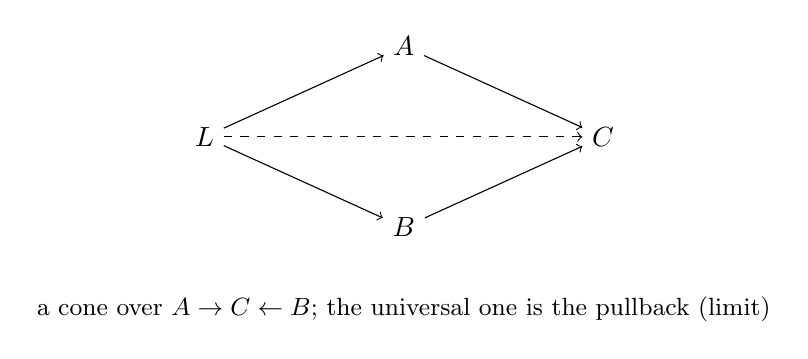
\begin{tikzpicture}[scale=1.15]
  \node (L) at (0,0) {$L$};
  \node (A) at (2.2,1) {$A$};
  \node (B) at (2.2,-1) {$B$};
  \node (C) at (4.4,0) {$C$};
  \draw[->] (A) -- (C); \draw[->] (B) -- (C);
  \draw[->] (L) -- (A); \draw[->] (L) -- (B);
  \draw[->,dashed] (L) -- (C);
  \node at (2.2,-1.9) {\small a cone over $A\to C\leftarrow B$; the universal one is the pullback (limit)};
\end{tikzpicture}
\caption{Limits are universal cones: compatible families, uniquely factoring. Colimits dualize:
gluing by identification.}
\end{figure}

\begin{remark}[Threads]
A sheaf (S26) is precisely a presheaf turning certain colimits of opens into limits of sets (the
equalizer axiom); \'etale spaces (S27) and topoi (S53) internalize this. Meanwhile
``object determined by its (co)cones of maps'' is the seed of Yoneda (\S4) and hence of
``point $=$ morphism'' (S29, S54).
\end{remark}

% ══════════════════════════════════════════════
\section{Adjunctions}
% ══════════════════════════════════════════════

\begin{definition}[Adjunction]
An \textbf{adjunction} $F\dashv G$ between $F:\mathcal A\to\mathcal B$ and $G:\mathcal B\to\mathcal A$
is a family of bijections $\Phi_{A,B}:\Hom_{\mathcal B}(F(A),B)\cong\Hom_{\mathcal A}(A,G(B))$
natural in $A$ and $B$. Equivalently: unit $\eta:1_{\mathcal A}\Rightarrow GF$ and counit
$\varepsilon:FG\Rightarrow 1_{\mathcal B}$ satisfying the triangle identities.
\end{definition}

\begin{example}[Adjunctions of the course]\label{ex:adj}
\begin{itemize}
  \item Free $\dashv$ forgetful: $\Hom_{R\text{-}\mathbf{Mod}}(R^{(X)},M)\cong\Hom_{\Set}(X,U(M))$ (S2).
  \item Abelianization $\dashv$ inclusion: $\Hom_{\mathbf{Ab}}(G^{\mathrm{ab}},A)\cong\Hom_{\Grp}(G,A)$.
  \item Tensor $\dashv$ Hom: $\Hom_R(M\otimes_R N,P)\cong\Hom_R(M,\Hom_R(N,P))$ --- the conceptual
    reason tensor is right-exact (Corollary~\ref{cor:adj-exact}); full use in S30.
  \item Sheaves: $f^{-1}\dashv f_*$ (S27); sheafification $a\dashv i$ (S27).
\end{itemize}
\end{example}

\begin{proposition}[Adjoints preserve (co)limits]\label{prop:adj-preserve}
A left adjoint preserves all colimits; a right adjoint preserves all limits.
\end{proposition}
\begin{proof}
Let $F\dashv G$ and $C=\colim_i D_i$ with cocone $D_i\to C$. For any $B\in\mathcal B$:
$\Hom_{\mathcal B}(F(C),B)\cong\Hom_{\mathcal A}(C,G(B))\cong\lim_i\Hom_{\mathcal A}(D_i,G(B))
\cong\lim_i\Hom_{\mathcal B}(F(D_i),B)$, naturally in $B$; hence $F(C)$ represents the cocone functor
of $(F(D_i))_i$, i.e.\ $F(C)\cong\colim_i F(D_i)$ by uniqueness of colimits
(Proposition~\ref{prop:limconstr}). The limit case is dual.
\end{proof}

\begin{corollary}[Right-exactness as a shadow]\label{cor:adj-exact}
Forgetful functors preserve limits (products and equalizers of rings/modules are computed on
underlying sets --- consistent with S1--S2); free functors and $-\otimes_R N$ preserve colimits
(coproducts and coequalizers) --- which is exactly the right-exactness of tensor proved in S2,
now explained: left adjoints preserve colimits but need not preserve limits, hence tensor can
destroy kernels (the failure measured by $\Tor$ in S43).
\end{corollary}

\begin{definition}[Representable functor; universal element]
$F:\mathcal A\to\Set$ is \textbf{representable} if $F\cong\Hom_{\mathcal A}(A,-)$ for some $A$; the
image of $1_A$ is the \textbf{universal element}. Products, kernels, and limits are representable
``cone functors''; this viewpoint is the gateway to Yoneda.
\end{definition}

% ══════════════════════════════════════════════
\section{The Yoneda Lemma (and a Remark on Monads)}
% ══════════════════════════════════════════════

\begin{theorem}[Yoneda lemma]\label{thm:yoneda}
For any functor $F:\mathcal A\to\Set$ and object $A\in\mathcal A$, the map
$\Psi:\Nat(\Hom(A,-),F)\to F(A)$, $\eta\mapsto\eta_A(1_A)$, is a bijection.
\end{theorem}
\begin{proof}
Inverse map: given $a\in F(A)$, define $\eta^a_X:\Hom(A,X)\to F(X)$ by $\eta^a_X(f)=F(f)(a)$.
Naturality: for $g:X\to Y$, $\eta^a_Y(g\circ f)=F(g\circ f)(a)=F(g)(F(f)(a))=F(g)(\eta^a_X(f))$.
Then $\Psi(\eta^a)=\eta^a_A(1_A)=F(1_A)(a)=a$. Conversely, for any $\eta$ and $f:A\to X$,
naturality of $\eta$ gives $\eta_X(f)=\eta_X(\Hom(A,f)(1_A))=F(f)(\eta_A(1_A))=\eta^{\Psi(\eta)}_X(f)$,
so $\eta=\eta^{\Psi(\eta)}$. Hence $\Psi$ is bijective.
\end{proof}

\begin{corollary}[Yoneda embedding]\label{cor:yoneda-emb}
The functor $\mathcal A\to[\mathcal A^{\mathrm{op}},\Set]$, $A\mapsto\Hom(-,A)$, is fully faithful;
hence $A\cong B$ iff $\Hom(-,A)\cong\Hom(-,B)$. An object is determined by its network of maps
into it --- equivalently, by its ``points'' $X\to A$ over all bases $X$.
\end{corollary}
\begin{proof}
Apply Theorem~\ref{thm:yoneda} with $F=\Hom(-,B)$ on $\mathcal A^{\mathrm{op}}$: 
$\Nat(\Hom(-,A),\Hom(-,B))\cong\Hom(A,B)$, and composition respects this identification; fully
faithfulness follows, and an isomorphism of representables yields an isomorphism of objects by
standard diagram chasing (the images of $1_A,1_B$ give mutually inverse maps).
\end{proof}

\begin{remark}[Where Yoneda becomes geometry]
S29 makes Corollary~\ref{cor:yoneda-emb} geometric: a scheme $X$ is determined by its functor of
points $T\mapsto X(T)=\Hom(T,X)$; ``$T$-valued points'' are morphisms, and non-representable functors
are moduli problems (S41). S54 repeats the pattern logically: a point of a topos $\mathcal E$ is a
morphism $\Set\to\mathcal E$. The proof above is all the machinery these deep theorems need.
\end{remark}

\begin{remark}[Optional: monads and comonads, in one paragraph]
A \textbf{monad} on $\mathcal C$ is $(T,\eta,\mu)$ with $T:\mathcal C\to\mathcal C$ and natural
$\eta:1\Rightarrow T$, $\mu:T^2\Rightarrow T$ (associative, unital); e.g.\ the free-group monad on
$\Set$, and --- the one that matters here --- the sheafification monad $a\circ i$ on
$\mathrm{PSh}(X)$, which is \emph{idempotent} ($\mu$ an isomorphism): algebras over it are exactly
sheaves (S27). Comonads dualize (e.g.\ forgetting-and-refreeing). Not used elsewhere in the course;
included so the remark in S27 has a home.
\end{remark}

% ══════════════════════════════════════════════
\section{Exercises}
% ══════════════════════════════════════════════
\begin{exercise}
Verify that a poset and a monoid, as in Example~\ref{ex:cats}, satisfy the category axioms; describe
functors between poset categories (monotone maps) and between one-object categories (monoid
homomorphisms).
\end{exercise}
\begin{exercise}
Show $\Hom(A,-)$ is a covariant functor and $\Hom(-,B)$ a contravariant one; write out both actions
on morphisms and check functoriality.
\end{exercise}
\begin{exercise}
Prove naturality of the double-dual map on finite-dimensional vector spaces and of abelianization
(Example~\ref{ex:nat}); give an example of a family of isomorphisms that is \emph{not} natural.
\end{exercise}
\begin{exercise}
Compute products and equalizers in $\Set$ and in $R\text{-}\mathbf{Mod}$ explicitly and verify the
universal properties; deduce Proposition~\ref{prop:limconstr} for these two shapes of diagram.
\end{exercise}
\begin{exercise}
Show $\Z_p=\varprojlim \Z/p^n$ satisfies the universal property of the limit in $\Ring$ (compatible
families of ring maps), and identify its elements with the $p$-adic series of S18.
\end{exercise}
\begin{exercise}
Describe the stalk $\mathcal F_x=\varinjlim_{U\ni x}\mathcal F(U)$ concretely as germs (pairs
$(U,s)$ modulo agreement on smaller opens) and verify the universal property of the directed colimit.
\end{exercise}
\begin{exercise}
Prove free $\dashv$ forgetful for $R\text{-}\mathbf{Mod}$ by writing the unit and counit and checking
the triangle identities; identify which adjunctions of Example~\ref{ex:adj} you can prove today.
\end{exercise}
\begin{exercise}
Prove directly (without Proposition~\ref{prop:adj-preserve}) that $-\otimes_R N$ preserves coproducts
and coequalizers; compare with the S2 right-exactness proof.
\end{exercise}
\begin{exercise}
Prove the Yoneda lemma (Theorem~\ref{thm:yoneda}) again from scratch, then deduce that any two
representations of a representable functor are isomorphic via a unique isomorphism compatible with
the universal elements.
\end{exercise}
\begin{exercise}
Show $G\mapsto G^{\mathrm{ab}}$ is left adjoint to the inclusion $\mathbf{Ab}\hookrightarrow\Grp$;
write the unit and counit; explain why this makes abelianization a colimit (a coequalizer).
\end{exercise}
\begin{exercise}
Identify each of the following as a limit or a colimit, and of which shape: kernel of a ring map;
cokernel; fiber product of schemes (S30); pushout of rings (gluing affines, S28); stalk; $\Z_p$;
$\bar\Q$ as a union of finite extensions.
\end{exercise}
\begin{exercise}[Optional]
Write down the free-monoid monad on $\Set$ explicitly (unit, multiplication) and verify the monad
laws; then explain why its algebras are exactly monoids --- the prototype of ``algebras over a
monad'' and of the sheafification remark.
\end{exercise}

% ══════════════════════════════════════════════
\section*{Where This Session Feeds the Course}
\addcontentsline{toc}{section}{Where This Session Feeds the Course}
% ══════════════════════════════════════════════
\begin{itemize}
  \item \textbf{Depends on:} S1 (primes for $\Spec$), S2 (modules, tensor, exact sequences),
    P1 (groups, abelianization), P3 ($\pi_1$ as a functor).
  \item \textbf{Feeds:} S16, S34 (inverse limits: $G_\Q$, profinite groups); S26--S27 (presheaves as
    functors, stalks as colimits, sheafification adjunction and monad, \'etale-space equivalence);
    S28--S30 ($\Spec$ functoriality, fiber products as pullbacks); S29 (Yoneda, functor of points);
    S41 (moduli as non-representable functors); S53--S54 (topoi, geometric morphisms, points as
    morphisms); S43 (tensor's left-adjointness as the reason for $\Tor$).
  \item \textbf{Unifying thread:} universal properties say an object \emph{is} its network of maps;
    Yoneda makes this a theorem; the course's ``point $=$ morphism into the object'' (S29, S54)
    is Yoneda applied to geometry and logic.
\end{itemize}

\subsection*{References for this session}
\begin{enumerate}[label={[\arabic*]}]
  \item Mac Lane, S. \emph{Categories for the Working Mathematician}, ch.I--V (selected).
  \item Leinster, T. \emph{Basic Category Theory}, ch.1--6 (gentle, complete proofs).
  \item Riehl, E. \emph{Category Theory in Context} (free; excellent on Yoneda and adjunctions).
\end{enumerate}

\vspace{1.5em}
\begin{center}
\rule{0.6\textwidth}{0.4pt}\\[0.5em]
\textit{End of Session S4 --- Act 0 complete; next: Act I, Session S5, Quadratic Residues and the Legendre Symbol}
\end{center}

\end{document}